\section{Chapter1 : Introduction} 

\subsection{ IOT IMPLEMENTATION PROJECTS }
This course is going to explain what IOT represents, what it consists of, also name some of the most important hardware which make it happen and try to give IOT a proper understanding of its meaning and importance.  The Internet of things has become a very widely spread concept in the last few years. The reason for this is mainly the need to computerize and control most of the surrounding objects and have access to data in real time. Think about parking sensors, about phones which can check the weather and so on.  The Internet of Things represents the whole way from collecting data, processing it, taking an action corresponding to the signification of this data to storing everything in the cloud. All this is made possible by the internet.  Let's take sensors as an example, they collect data and send it to a processing device, which will perform the convenient actions. Then, the data will be stored locally and, by using the internet, it is subsequently sent out to the cloud. The problem here is that the data stored in the cloud is sometimes not useful. There is not enough local processing happening before data is saved in the cloud.  The ideal scenario, towards which the Internet of Things is headed, would be to have a computer store data locally, process it, check for abnormalities or search for relevant segments and upload only this information to the cloud. This concept is called either Edge, according to Intel, or fog computing as stated by Cisco, implying what happens before the cloud.  The IOT is involved in medicine, agriculture or transportation due to sensors and cloud storage.
IOT Stack a basic Internet of Things system consists of the following components:  

\begin{figure}[ht]
    \centering
    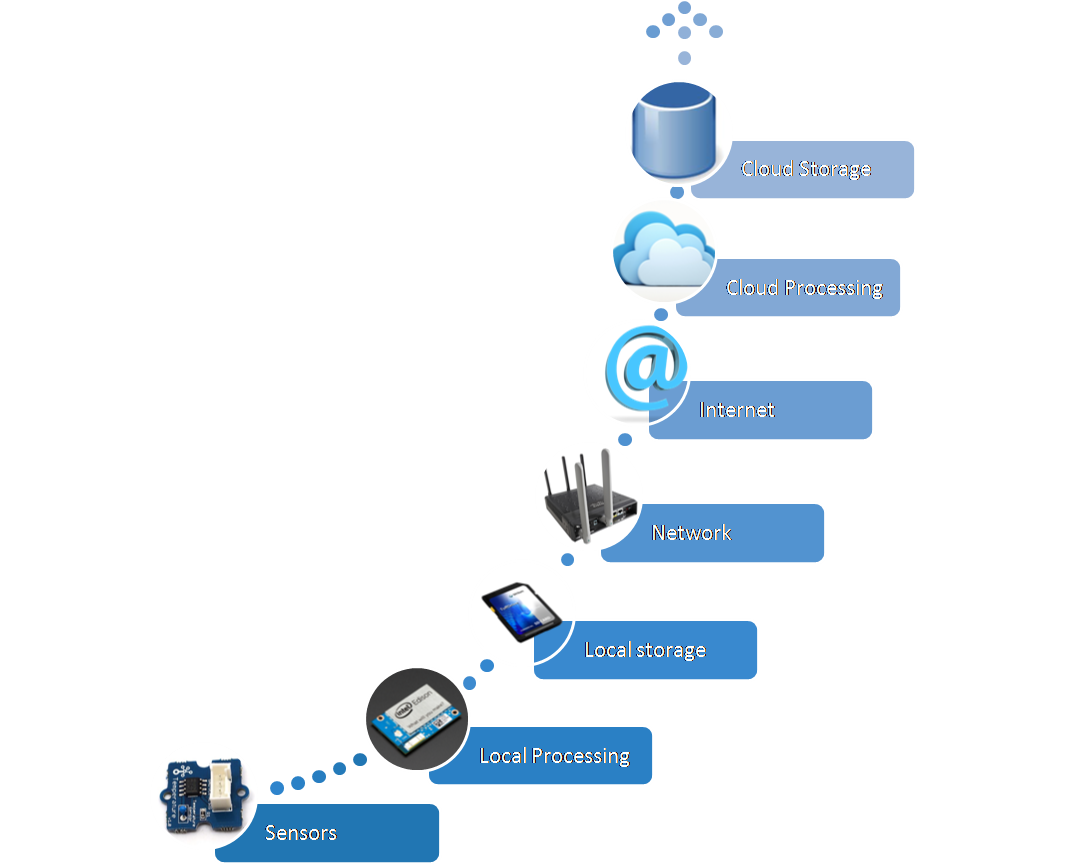
\includegraphics[width=0.3\textwidth]{figures/IOT.png}
    \caption{IOT}
\end{figure}

\subsection{Sensors}
They transform analog data given from scanning the environment to digital data, but they merely do any processing. On the bright side, they don't consume much power and can live on batteries for a long time. Sensors are present in everyday life more than you would expect.  
They improve industry, agriculture, homes, transportation or smart phones for example. They are tools which help monitoring the environment, collecting data about it and, with the help of computers, acting accordingly. 

\begin{figure}[ht]
    \centering
    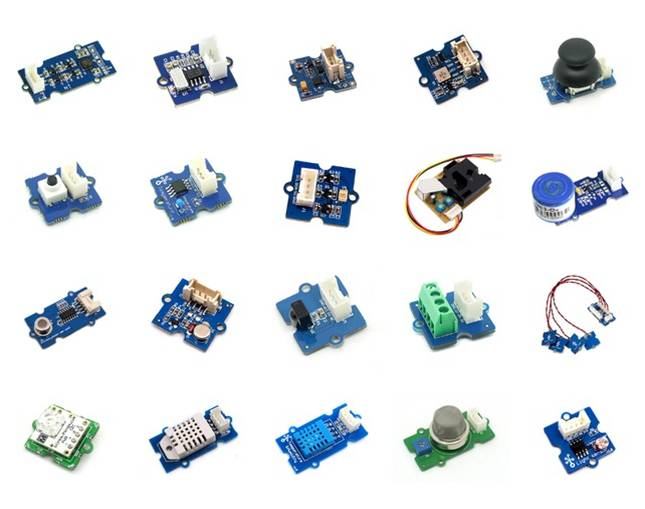
\includegraphics[width=0.4\textwidth]{figures/Sensors.jpg}
    \caption{Sensors}
\end{figure}

\subsection{Local processing and storage devices}
 Local processing devices are the second level and third in IOT. At this point, data is locally stored and processed, ideally not sent forwards unless relevant. This part is explained in detail in the hardware section, as said devices are nothing more than microcontrollers and embedded boards, which handle the data they receive from the sensors.  
 
\subsection{Network and Internet}
There is hardware which connects to the previously described devices, pulls out data and sends it to the cloud to be stored. There are 4 protocols used at this level: CoAP, MQTT (less secure and designed for machine to machine communication), HTTP (web protocol) and XMPP which functions as a chat.

\subsection{Cloud} 
In the cloud, which comes next, data is collected and the main goal is for it to reach the point of making predictions based on the stored information. The cloud however, even though it represents one of the most useful features of the internet, is not used properly. Data sent to the cloud didn't reach the level of being formerly processed. Which means there is no preselected data? The cloud is constantly loaded with irrelevant information and thus losing its property of being practical.

\subsection{Hardware} 
An important subject concerning the IOT is open hardware. The designers of such hardware publish the schematics which, when the current started, were a real boost for the IOT.   

\subsection{Microcontrollers}  
Microcontrollers were the first one to appear as an option for developers. They are small computing devices, easily connectable to hardware. The development tools were, however, an obstacle and made using them very complicated.  
The first easy to use microcontroller was Arduino. It is a small programmable device, on which you can run simple, open source software called firmware. The only fault was that it didn't have enough processing power and, as a result, no more than 4 network connections were supported. It’s RAM being of 2KB. Shortly, the Arduino does not run an Operating System, what it runs is called Firmware. Basically, it runs only one program. The result is that you can estimate what program sequence gets executed at a certain time. Program written to the Arduino remain there until they are replaced with another program. Even when powered off, Arduino stores 

\begin{figure}[ht]
    \centering
    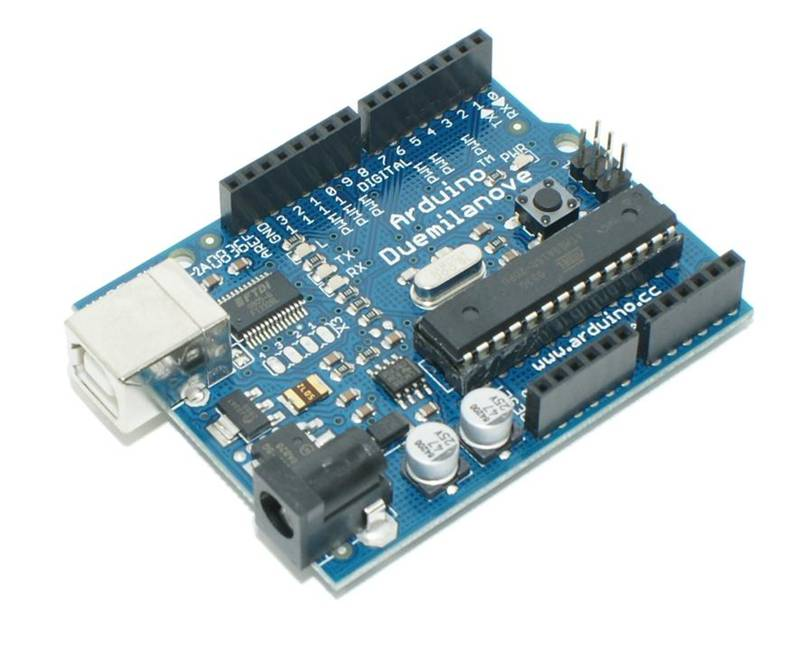
\includegraphics[width=0.3\textwidth]{figures/Microcontroller Kit.jpg}
    \caption{Microcontroller Kit}
\end{figure}

All the above sections were talking about the hardware and its components ... while about its software :

\subsection{Computers}
Conversely, since it is a computer, the Raspberry Pi runs an Operating System. That means that you can run multiple programs on it and you can run applications that use Internet services. However, this also implies that the application you run on the Raspberry Pi is not real time, thus you cannot estimate when a certain sequence will get executed. Raspberry Pi came second with the qualities of being cheap and useful. It is actually a small computer, it runs Linux as operating system and has a full network system, solving thus the processing problem of the Arduino.

\begin{figure}[ht]
    \centering
    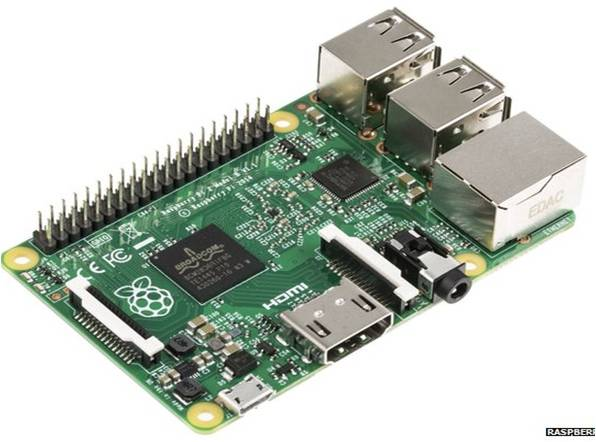
\includegraphics[width=0.3\textwidth]{figures/Raspberry Pi.jpg}
    \caption{Raspberry Pi}
\end{figure}

\subsection{Development devices}
The appropriate hardware can be found by checking many aspects. There are many boards, but they are good for different kinds of projects.  
For sensor handling Arduino, ChipKIT and LounchPad are the best options.  

\begin{figure}[ht]

\begin{subfigure}{0.5\textwidth}
    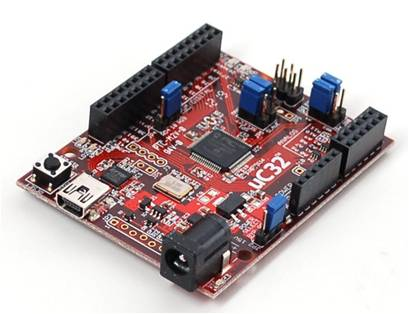
\includegraphics[width=0.9\linewidth, height=5cm]{figures/ChipKIT.jpg}
    \caption{ChipKIT}
\end{subfigure}
\begin{subfigure}{0.4\textwidth}
    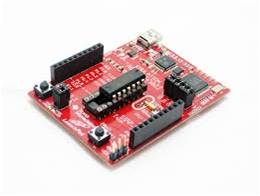
\includegraphics[width=0.9\linewidth, height=5cm]{figures/LounchPad.jpg}
    \caption{LounchPad}
\end{subfigure}

\caption{Sensor Handling Boards}
\end{figure}

For processing: the STM32 with 128KB of RAM, Particle with an ARM chip and Wi-Fi, Espino which is actually a JavaScript machine and so, you can write JavaScript code to run on it.

\begin{figure}[ht]

\begin{subfigure}{0.4\textwidth}
    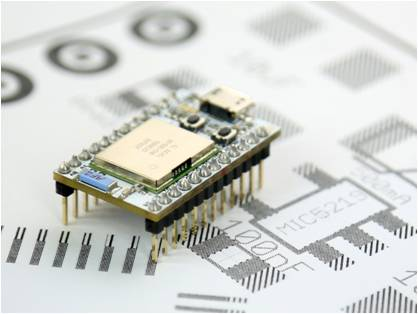
\includegraphics[width=0.9\linewidth]{figures/Spark Core WIFI Board.jpg}
    \caption{Spark Core WIFI Board}
\end{subfigure}
\begin{subfigure}{0.5\textwidth}
    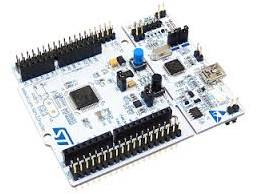
\includegraphics[width=0.9\linewidth, height=5cm]{figures/Nucleo STM32F4.jpg}
    \caption{Nucleo STM32F4}
\end{subfigure}

\caption{Boards for processing STM32}
\end{figure}


For processing and network, there are the Raspberry Pi; Intel Galileo which handles hardware pretty good, has 256MB of RAM and a Quark processor; The Intel Edison which comes as an improvement to the Galileo, can be used with Wi-Fi and Bluetooth and has a 4GB flash memory; Beagle bone Black also brings flash memory; UDOO Neo is a combination of a Raspberry Pi and an Arduino, project started on Kickstarter; Parallels which is very different from the others, being a prototyping board, plus, it has a chip which processes 16 or 64 programs at a time 

\begin{figure}[ht]
    \centering
    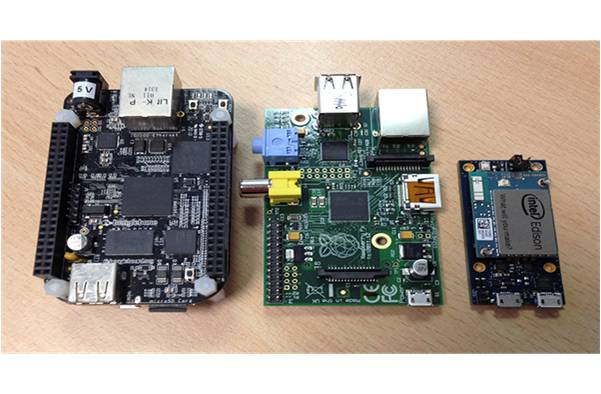
\includegraphics[width=0.4\textwidth]{figures/Embedded Linux Boards.jpg}
    \caption{Embedded Linux Boards}
\end{figure}

\subsection{Software}
 Prototyping is a necessary process while building a professional product. The software used for it should be fast to write, easy to deploy when finished and it’s there to make a proof of concept. However, it is not supposed to be user level grade.  
Prototyping has the only property of making a statement, whereas professional programming can’t have any faults, can’t break and has to meet the client’s needs. The software’s built for this job are Eclipse, VIM, MBED- online platform where you can write the code and download the binary file for the board-, Intel XDK which uses JavaScript as language for developing and also offers HTML as an alternative.
 The field of data acquisition and analysis brings: 
 Lively, which collects data and displays it, offers libraries for you to integrate into your project, send the latter to the cloud. Here, you can add graphs and monitored everything.
 Microsoft Azure, through which you push data to the cloud with failure detection as target. With this software, there’s no need for machine learning algorithms when you can use Microsoft’s technology and knowledge to build prediction models.  
Solution builders such as Wyliodrin allow prototyping and build solution projects to be sent to the clients.

\begin{figure}[ht]
    \centering
    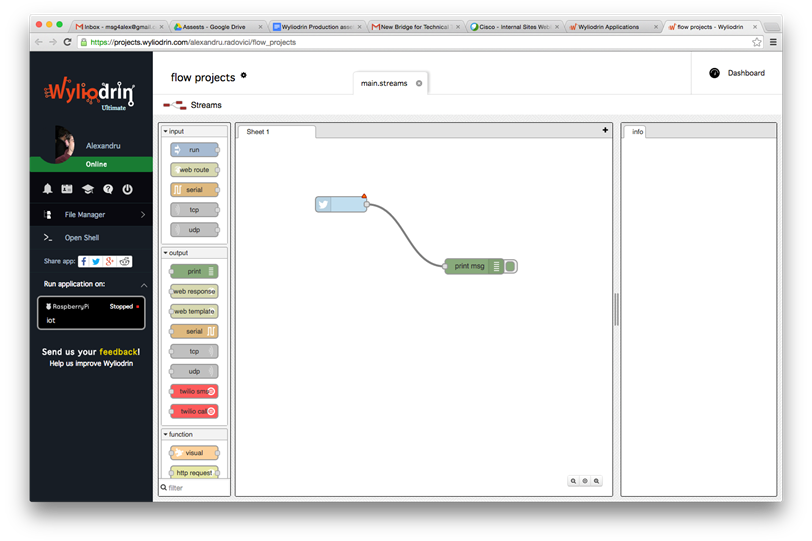
\includegraphics[width=0.4\textwidth]{figures/Wyliodrin Studio.png}
    \caption{Wyliodrin Studio}
\end{figure}

\textbf{Sensors and peripherals}
Slides are available from the link  
This course will go through both analog and digital sensors, describing how they function and different ways of connecting and using them. More than this, it will present some other important peripherals, from the basic ones: LEDs to be more complicated - shift registers or significant ones- LCDs.  

\subsection{Sensors}
Sensors are devices that scan the environment and get data from it. Some examples of sensors are: thermistors, buttons (because they send a value, sensing the environment), photo resistors, infra-red sensors, distance sensors.  
Types of sensors:  
Analog Sensors - send an analog value that needs to be processed by the ADC 
Digital Sensors - send a digital value 
Basically, all the sensing parts are analog.  
For the analog sensor the sensing part is directly connected to a micro controller. They are easy to interface; you only need an ADC to do some computing to find the real value.  
Digital sensors are more complicated because the micro controller that processes the data is already in the box of the sensor and it sends the data out on a communication channel that implements some type of protocol. In order to get the data, the device needs to communicate with the sensor via the protocol.  

For the analog sensors there are two types: with two or three pins. 
 An analog sensor will most probably be connected as a voltage divider. Such a sensor has a variable resistance, according to a specific environment element. Take a light sensor as an example: the more light there is, the lower the resistance. For the temperature sensor, the higher the temperature, the lower the resistance. You practically measure the voltage drop in the circuit. The 2 leg and 3 leg analog sensors are mentioned above. The sensors that have 3 pins usually have the voltage divider already integrated: one pin goes to VCC, one to the Ground and the third pin goes to the analog input. For the sensors withe 2 legs, you have to build the voltage divider yourself by adding a resistance to the circuit.
 If you switch VCC with ground, some sensors will burn.  
Another particularity of the sensors is that they will introduce some errors in the measurements, depending on the quality of the sensor. These parts usually increase in accuracy if they have the voltage divider inside as they bring some corrections. More to this, the sensors are not linear.  
One simple way to connect errors in reading or the ones that occurred due to the fact that the circuit is not perfect is to average them (usually using 1000 samples). This works on micro controllers, but on computer boards, it might result in reading the same value over and over.  

\subsubsection{Button}
It is one of the simplest sensors that you can connect. It is in fact an analog sensor, but it can only report 2 values: either 1 or 0. If the button is released, the resistance is infinite, if it is pressed, the resistance becomes 0 and the input will be directly connected to the ground. 

\begin{figure}[ht]
    \centering
    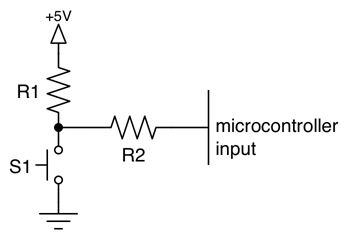
\includegraphics[width=0.4\textwidth]{figures/Button.png}
    \caption{Button}
\end{figure}

The button becomes a pull-up resistor because when the button is not pressed it pulls up the voltage up to 5V. You need a really small resistor so that when the button is in the air the voltage drop will be insignificantly low, so that you can still read 5 volts. The problem comes up when you press the button for a longer period of time. In conclusion, you need a resistor sufficiently high that you won’t drain the source too fast, but sufficiently low to be able to read the value 1.  
If R1 is replaced by S1 it will be called a pull-down resistor: it will pull down the voltage from that point to the ground the moment the button is not pressed. When the button is pressed it will stop the current from flowing too fast and having a short circuit. The input will be connected to VCC.  

\subsubsection{Button Denounce}
This problem is really visible on micro controllers because they sample fast. Buttons are imperfect, so from the moment you start pressing the button, there is a short time when the button’s connectors start approaching and the distance is really small resulting in an electric discharge. The resistance will be neither 0, nor infinite, so for a short period of time the resistance will vary.

\begin{figure}[ht]
    \centering
    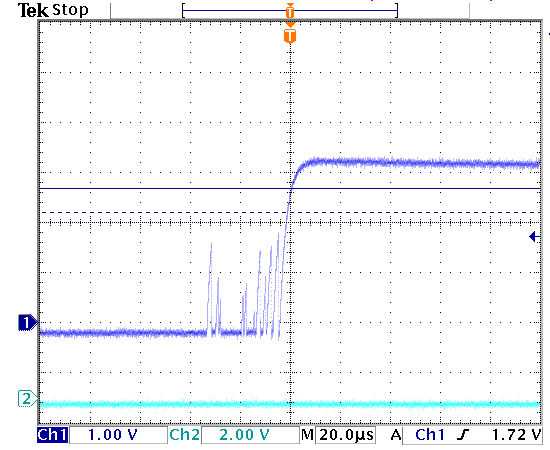
\includegraphics[width=0.4\textwidth]{figures/Button Denounce.png}
    \caption{Button Denounce}
\end{figure}

With the microelectronics, you will see many values of 1 and 0 continuously changing. One way to denounce is to average the values and if the result is different from 0 or 1, then to discard the measurement because the button bounced. Another way is to use a trigger which, for an amount of time won't read any other value thus not detecting the edges. Expensive microcontrollers have denouncing circuits.  

\subsubsection{Potentiometer}
A potentiometer is a variable resistance, with 3 pins. Usually it is a full resistor and the pin is connected in the middle (it can float around the full resistor and split it into two resistors so it works as a voltage divider). You can connect it in two ways: either by making a voltage divider, choose R1 and connect two of the pins in the voltage divider (the middle one and one of the extremities), or by connecting one pin to VCC, one the Ground and the middle one to the input. To have a linear function as input from the sensor some computing is requested.  

\subsubsection{Thermistor}
Let's see an example of how an analog sensor can be connected to a board and how an application looks in Visual Programming for the thermistor, for instance. This sensor is still a variable resistor that changes its value with the temperature. You can compute the actual temperature using that value and a formula that takes into account the thermistor`s parameters, among which the resistance at 25 degrees. This kind of sensor has a low accuracy and is used to get a rough idea about the temperature. 

\begin{figure}[ht]
    \centering
    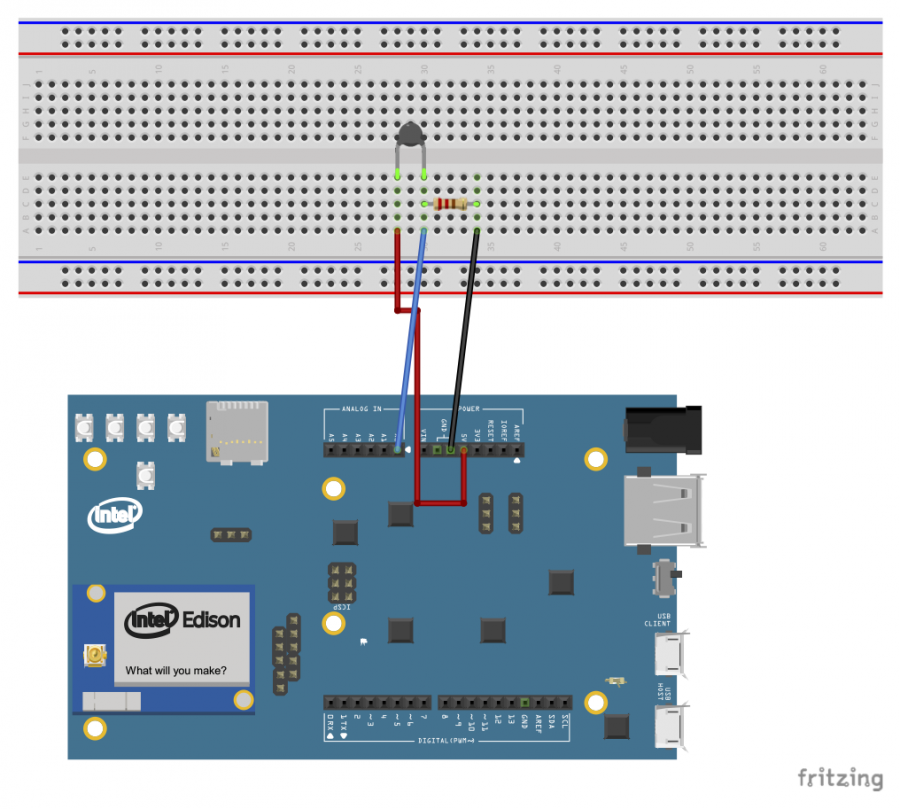
\includegraphics[width=0.4\textwidth]{figures/Thermistor connection.png}
    \caption{Thermistor connection}
\end{figure}
\begin{figure}[ht]
    \centering
    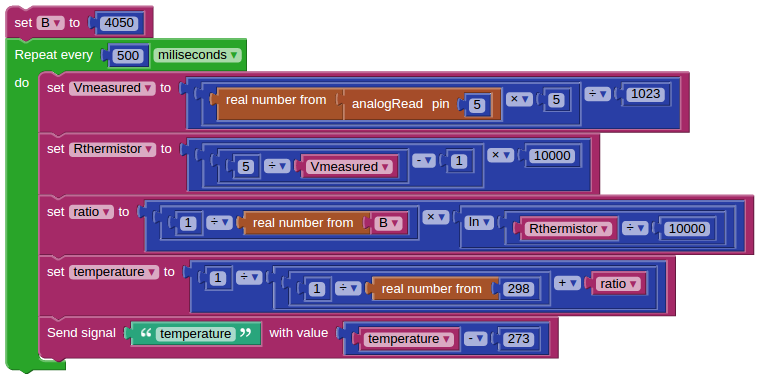
\includegraphics[width=0.4\textwidth]{figures/Thermistor in programing.png}
    \caption{Thermistor in programing}
\end{figure}

\subsubsection{Temperature sensor}
Note that there is a difference between the two sensors, consisting of the fact that the temperature sensor has a linear resistance-temperature characteristic, while the thermistor usually has the output voltage as a logarithmic or exponential function. Also the formulas to find the temperature in Celsius degrees are different.

\subsubsection{Light Sensor}
This is also a resistance that changes its value due to the amount of photons it receives. Measuring the voltage drop on the resistance, you can get an idea about the light intensity. How does it actually work? If there is much light, there will be many photons in the photocell, thus less electrons to stop the electric current, which means the resistance of the sensor is lower.

\begin{figure}[ht]
    \centering
    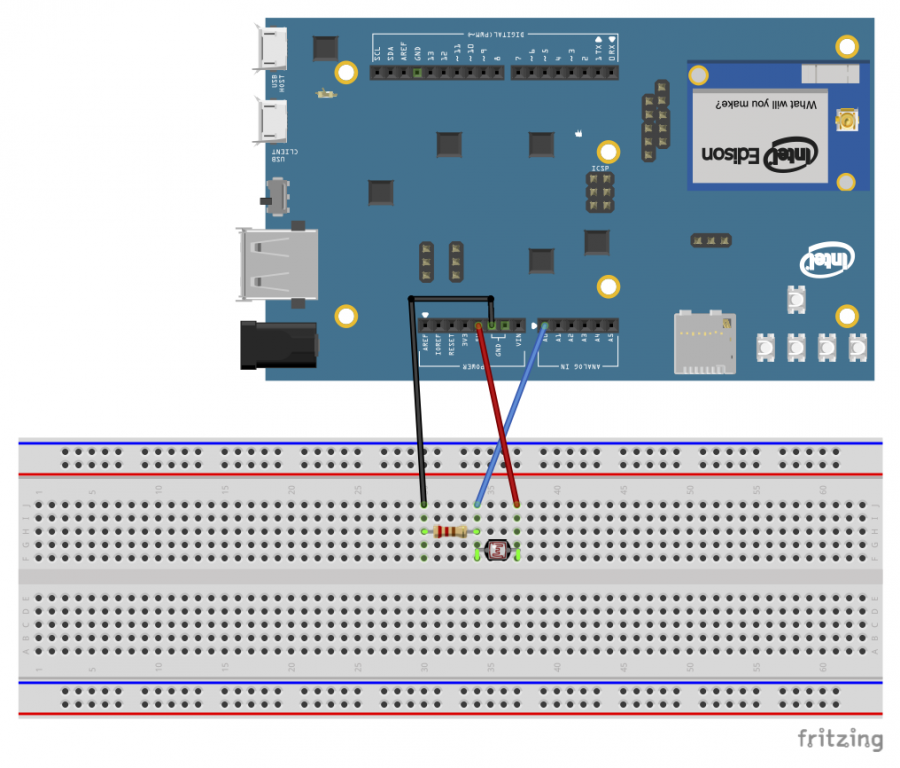
\includegraphics[width=0.4\textwidth]{figures/Light Sensor connection.png}
    \caption{Light Sensor connection}
\end{figure}
\begin{figure}[ht]
    \centering
    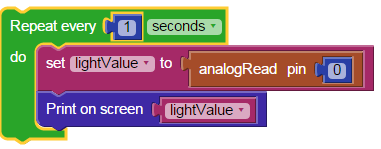
\includegraphics[width=0.4\textwidth]{figures/Light Sensor in programming.png}
    \caption{Light Sensor in programming}
\end{figure}

\subsubsection{Gas Sensor}
This sensor detects CO2. Pay attention that in order to detect gas it uses an exothermic chemical reaction therefore it heats up so don`t touch it while it is connected to the board. More importantly pay attention that this sensor IS NOT for safety-important applications.

\subsubsection{Distance Sensor}
This sensor works like sonar. It has 4 pins. Two of them are the power pins: GND and VCC, and the other two are the trigger and the echo pins. The trigger will send out an ultrasonic signal and wait for the response. The moment the signal is sent out, the echo pin is 1, when the response comes, this pin turns to 0. The distance is measured by multiplying the time needed for the response to come with the speed of sound.  Another type of sensor is an infrared one. It has an ADC inside so computing the distance is after a simple formula.

\subsubsection{Digital sensors}
Digital sensors work with either of the two protocols: SPI or I2C.

\subsubsection{SPI}
This protocol involves several slaves and a master. The communication is always initiated by the master. The pins for such a sensor are SS (slave select), MISO, MOSI, Clock, each with their role.  MOSI stands for master out, slave in, which means that a line is created to send data from the master to the slave. MOSI is the line that facilitates the communication in the opposite direction: the slave writes on the line and the master samples. 
The master is the one who generated the clock. SS pin will be 0 when the slave is active and conversely 1 when the slave is inactive. In the first case, the slave waits for the clock to transfer data. One master has pins for each slave, but it can’t work with more than one slave at a time, since the MISO and MOSI lines would get impossible to use.  
Communication in this protocol is always an exchange. 

\begin{figure}[ht]
    \centering
    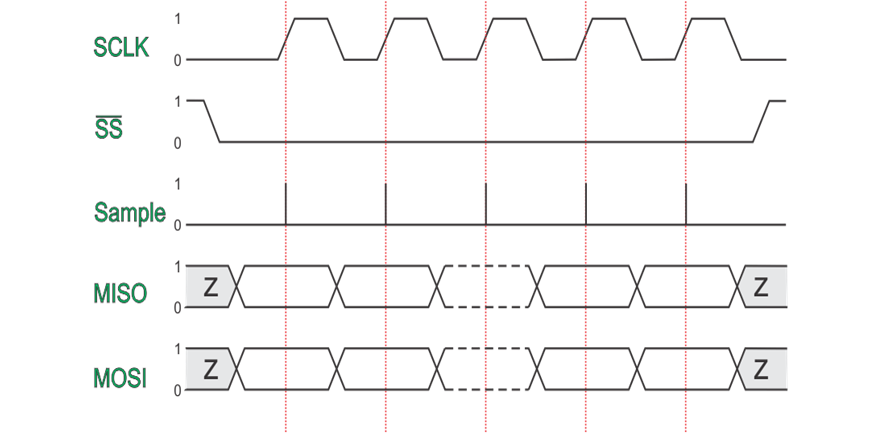
\includegraphics[width=0.4\textwidth]{figures/SPI.png}
    \caption{SPI}
\end{figure}

\subsubsection{I2C}
This protocol works with one master and several slaves as well. This time there is no slave selection, but each slave has a fixed address.  
It only uses two lines: SDA and SCL: serial data and serial clock line. This protocol is called a half-duplex as it only uses one line for communication. The transfer of data goes as follows. The master sends the address. The slave identifies itself, sends out and acknowledgement message, and then the master writes or reads the data, all this on the same line.  

\begin{figure}[ht]
    \centering
    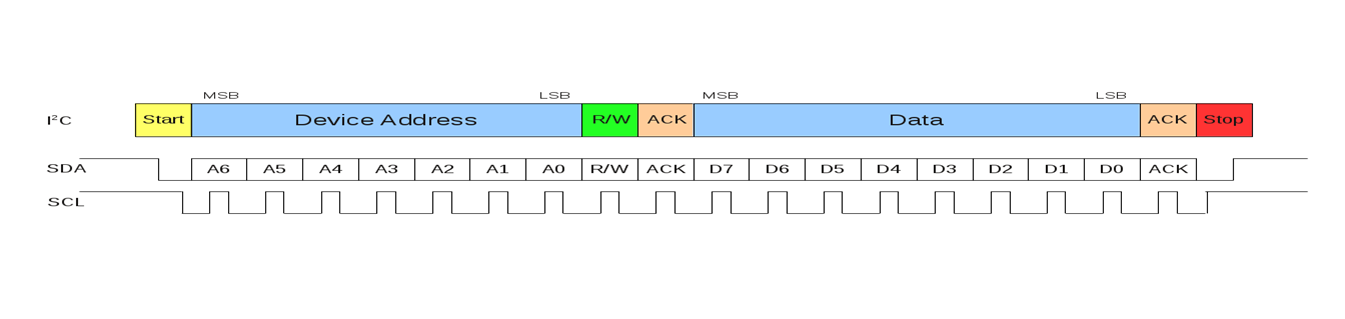
\includegraphics[width=0.4\textwidth]{figures/I2C.png}
    \caption{I2C}
\end{figure}

In general microcontrollers can be masters or slaves, but the computers can only be masters. Accelerometer and Gyroscope 
See below an example of wiring and programming for a digital sensor.  
Using this sensor, you can determine acceleration on all three axes and also the rotation angle. An important note is that it also measures gravitational acceleration so don`t be surprised to get values different from 0 when the sensor is not moving.  

\begin{figure}[ht]
    \centering
    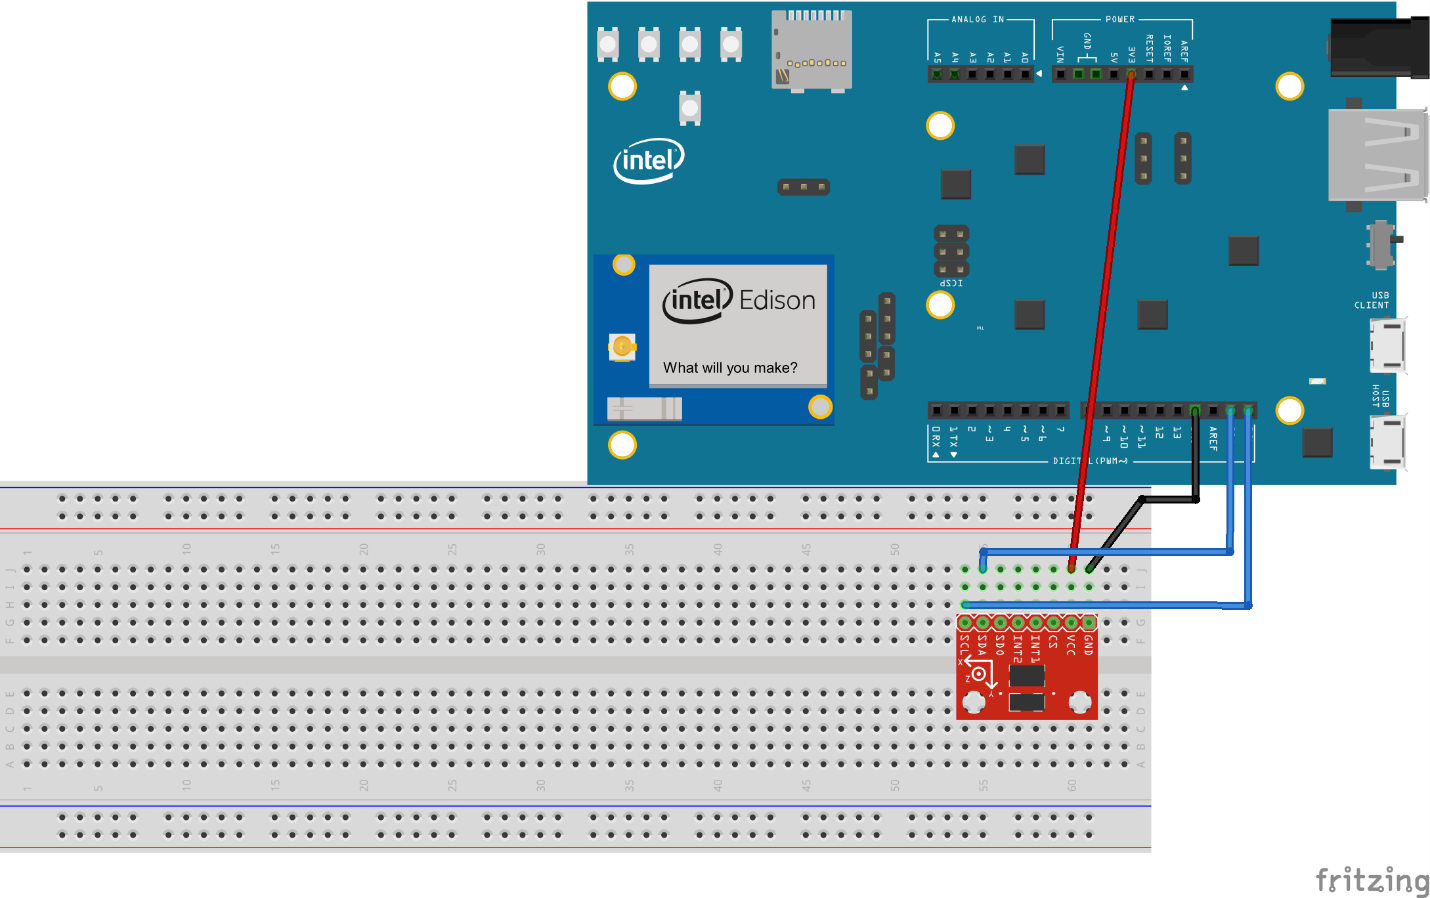
\includegraphics[width=0.4\textwidth]{figures/I2C connection.png}
    \caption{I2C connection}
\end{figure}
\begin{figure}[ht]
    \centering
    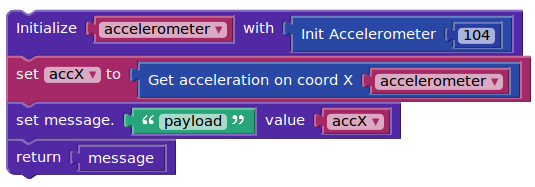
\includegraphics[width=0.4\textwidth]{figures/I2C in programing.png}
    \caption{I2C in programing}
\end{figure}

\subsection{Peripherals}
Peripheral device, also known as peripheral, computer peripheral, input-output device, or input/output device, any of various devices (including sensors) used to enter information and instructions into a computer for storage or processing and to deliver the processed data to a human operator or, in some cases, a machine controlled by the computer. Such devices make up the peripheral equipment of modern digital computer systems.

\subsubsection{LED}
An LED is a light emitting diode. A diode allows the current to pass only in one direction. Also, it has no resistance, which means it will be in a short circuit once it is wired to a circuit with no resistor. You will see when you look at the LED that it has two legs. One is longer, that one is usually the anode. This one has to be connected to the GPIO pin of the Edison. The shorter leg should to be connected to the resistor and then to the ground pin of the board.  
Although the position of the resistor is not fixed, it can either connect the ground to the cathode or the anode to the GPIO pin, the cathode should be connected to the ground to obtain the usually desired behavior. That means that we want the LED to light when the GPIO is set to HIGH and not to light when the GPIO is set to LOW. If you put the legs the other way around, the effect will be the opposite.  

\subsubsection{7 segment display}
It is an electronic component consisting of 7 LEDs. These have either a common cathode or common anode. In the first case, the LEDs need the value 1 on the pins to be alight, but in the second case, the VCC will be common. The latter situation means that the LEDs are alight when the value on the pins is 0.

\begin{figure}[ht]
    \centering
    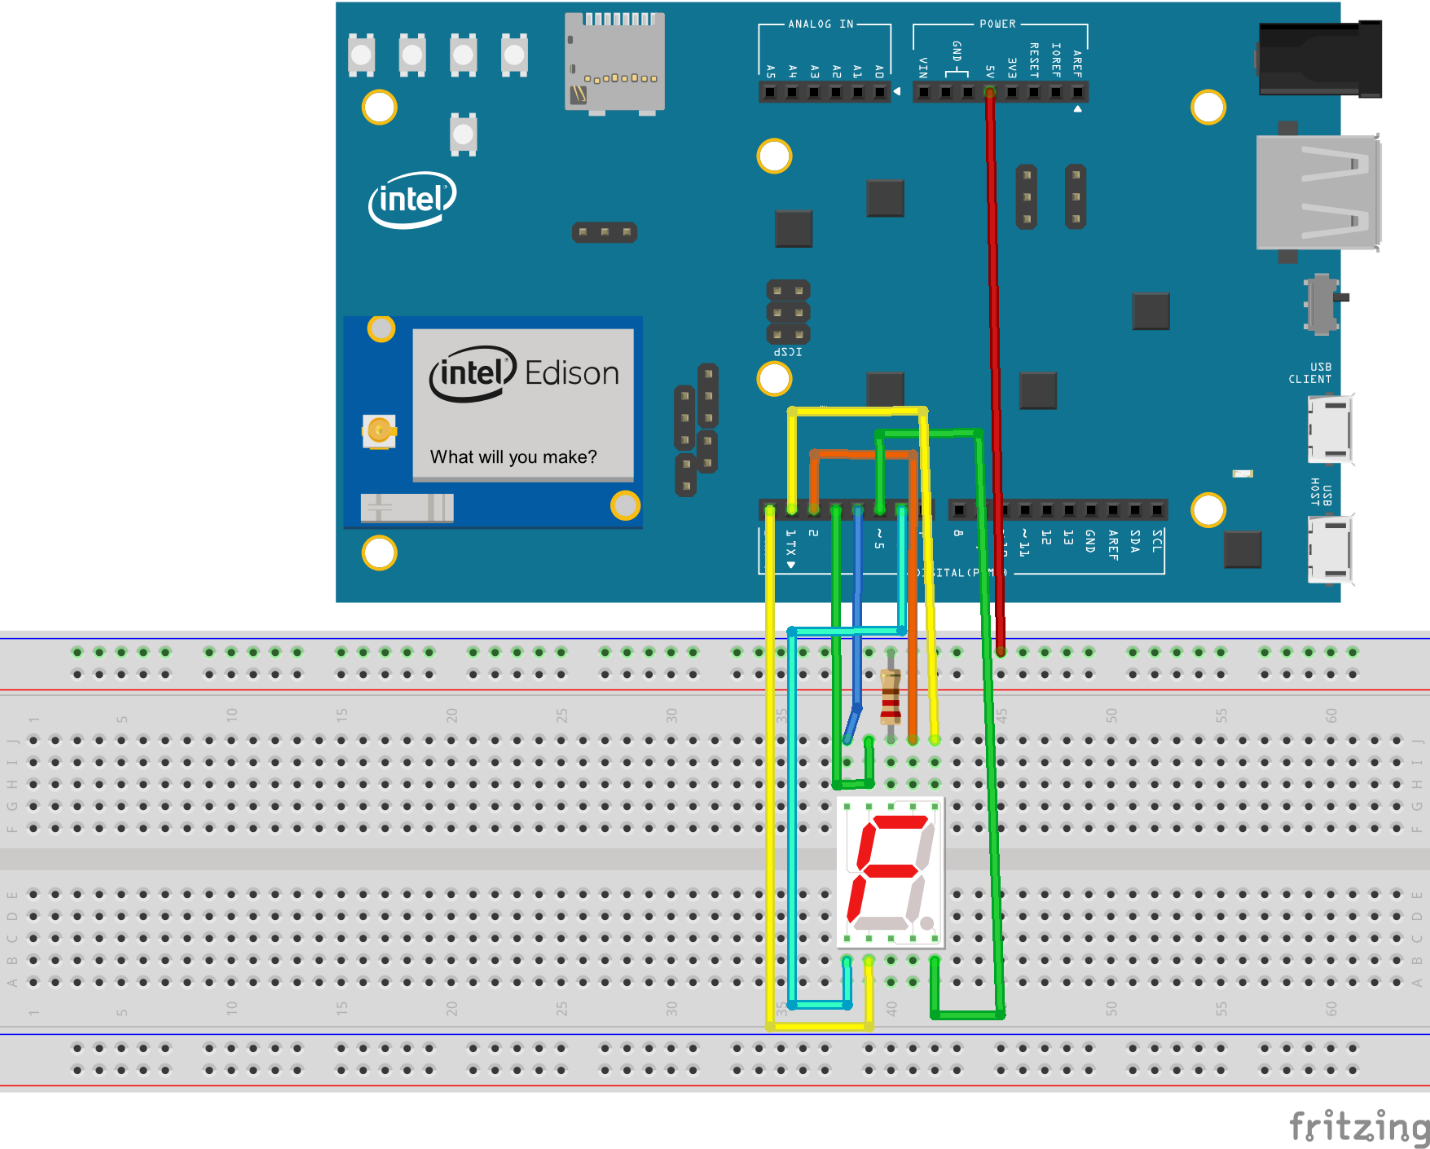
\includegraphics[width=0.4\textwidth]{figures/7 segment display connection.png}
    \caption{7 segment display connection}
\end{figure}

How do you connect it?  In visual programming, there are special blocks for the piece. All you have to do is to look up your model's Data sheet AND insert the number of the pins for each segment.  

\begin{figure}[ht]
    \centering
    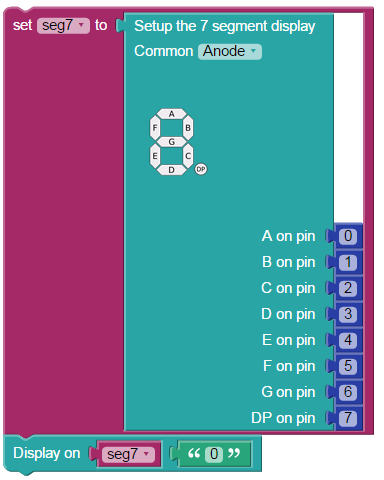
\includegraphics[width=0.4\textwidth]{figures/7 segment display in programing.png}
    \caption{7 segment display in programing}
\end{figure}

\subsubsection{Shift register}
It is a serial to parallel register. Being a register, it is actually a memory. The data stored inside goes from QA to QH. These are the GPIO pins. OE stands for output enable, it is used to disconnect the pins all at once. SER is the serials input pin, RCLK latch clock, SCLK is the serial clock and SRCLR is the clear pin. The data is easy to read, paralleled, but written by shifting it inside. When the serial clock switches from 0 to 1 the register reads the value in the SER, puts the value from QH into QH, QG into QH and so on until it's QAs turn to go into QB and SER is now stored into QA. You would need 8 cycles to change all the values from a register. The bits can be read all at a time, but not written this way.  
Two shift registers can be connected together.  
A shift register offers 8 outputs using only 2 lines: the clock and the SER. When SRCLR is 1, everything is cleared out. The shift register changes the values in the output as others come in, so this can be visible. To avoid this problem, good quality shift registers have a parallel to parallel register. This means that only when a cycle is complete the RCLK will switch and the values are given as output. This is why the latch clock is needed. 

\begin{figure}[ht]
    \centering
    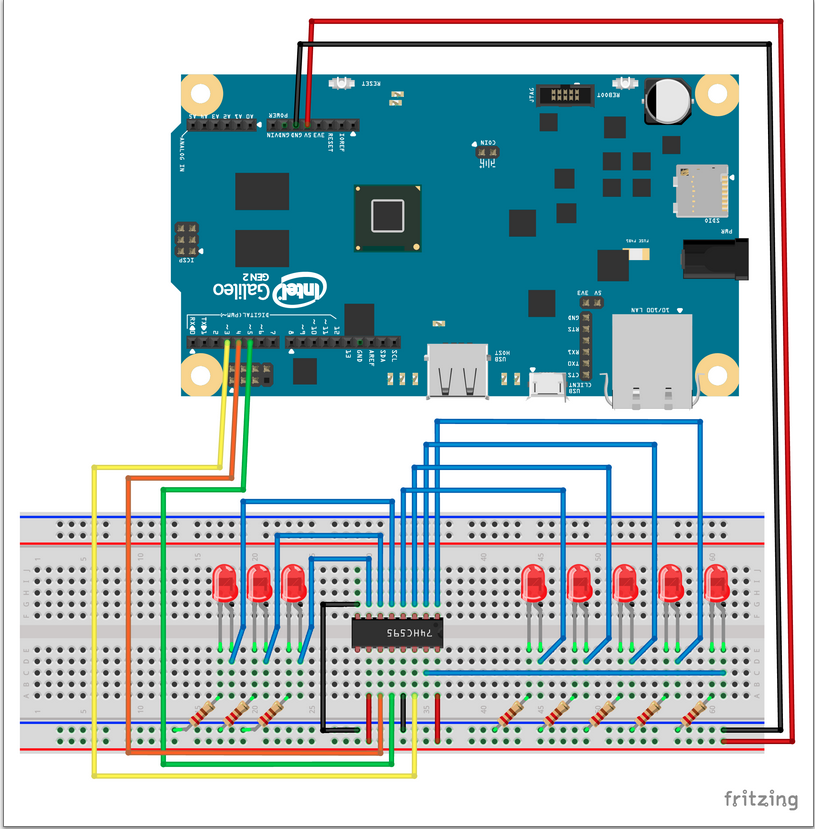
\includegraphics[width=0.4\textwidth]{figures/Shift register connection.png}
    \caption{Shift register connection}
\end{figure}
\begin{figure}[ht]
    \centering
    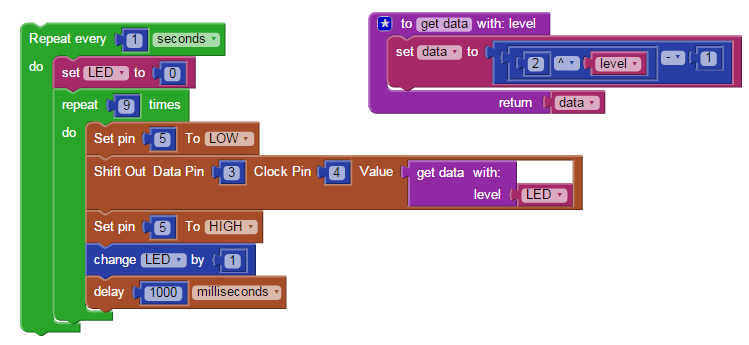
\includegraphics[width=0.4\textwidth]{figures/Shift register in programing.png}
    \caption{Shift register in programing}
\end{figure}

\subsubsection{LCD}
An LCD with 16 colons and 2 rows needs 16 pins to be controlled. It can use either a 4 pin protocol or an 8 pin protocol. The former will need 12 pins and the last, all the 16 pins. There are 4 power pins, meaning two groups of GND and VCC, one group being used by the backlights. Any LCD uses a potentiometer to set the contrast. The enable pin of an LCD can be connected to the ground or to a microcontroller. There are also I2C LCDs that work with only 4 pins, have an integrated potentiometer and can be connected in the same circuit only if they have different addresses.  

\begin{figure}[ht]
    \centering
    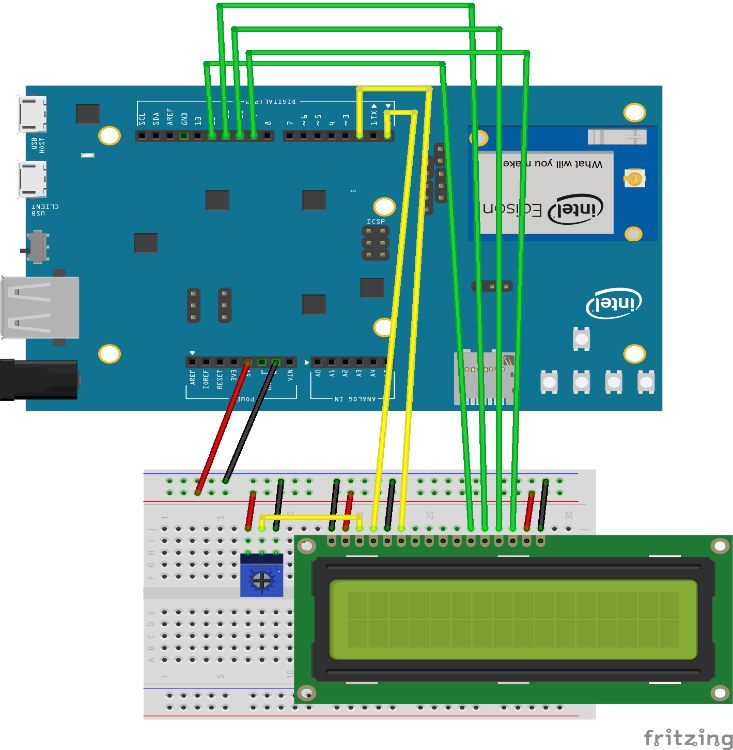
\includegraphics[width=0.4\textwidth]{figures/LCD connection.png}
    \caption{LCD connection}
\end{figure}
\begin{figure}[ht]
    \centering
    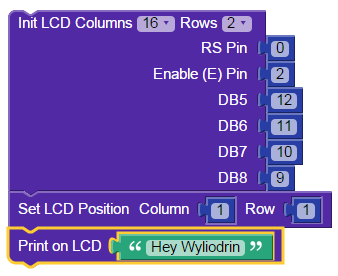
\includegraphics[width=0.4\textwidth]{figures/LCD in programing.png}
    \caption{LCD in programing}
\end{figure}

This course explains what a web server is, how it works, protocols used in web programming and gives examples on building and implementing a web server, of creating dynamic web pages. It also introduces the students to AngularJS and JQuery.  

\subsection{Web server and HTTP}
Any computer that can implement http or https is able to play the role of a web server. HTTP is a protocol, a way of communication which supplies web pages. It is pretty widely used and easy to implement. Through http you can transfer HTML and create simple user interfaces, it can implement Java Script and make more complicated web pages and it is available in most of the browsers. One of the great qualities of this protocol is that it replaced complicated and heavy displays with user friendly web pages.  
How does it work? The browser sends a request to the server who searches the demanded page and returns it to the browser for the user. The request will consist of information about the kind of browser that is used, about the computer or about the document requested. It will have a method, a URL, a query string and the upload body in case you want data to be sent to the server.  
The response will include the status, which tells the browser if the page was found or not (the errors among the 400s are about a not found page, 300 are redirections and 200s are confirmations of the page being found). 

\begin{figure}[ht]
    \centering
    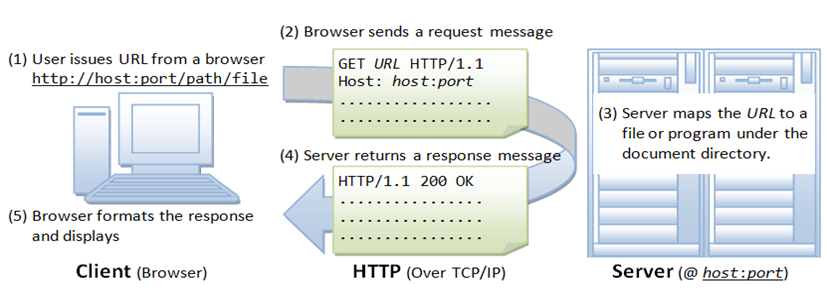
\includegraphics[width=0.4\textwidth]{figures/HTTP.png}
    \caption{HTTP}
\end{figure}

\textbf{HTTPs has two important security roles. }
\begin{itemize}
\item It encrypts the data. The request and the response will be both encrypted on sending and decrypted when read. 
\item The server is always asked for a certificate of authenticity before it is asked for a page. This prevents against stolen data through false web pages.  
\end{itemize}

What does a query consist of? It will always look like this: http://address: [port] URL ? querystring. The port can be absent, in which case it will be 80 for http and 443 for https. It has to be specified if it is not one the two. Concerning the URL, when it is not written, the default will be /. The available methods in http are: get, post, put and delete. The main ones being the first two.  

\begin{itemize}
\item Get method needs no upload body. It will only ask for data from the server and send only the headers, the address, the URL. 
\item Post sends important data to the server, which will be uploaded. Post has the role of modifying data on the server. The response of both these methods is the page and any additional information that was requested.  
\item Put is similar to post, only that in the semantic way, this method only creates an object on the server. 
\item Delete also plays a semantic part. It needs no upload body and it deletes objects on the server. The same action can be performed however using get. 
  
\end{itemize}

On one server there can be more than one websites, which means that, if the host is not specified in the request, the response may not be the one the browser expects.  
Also, the response may have more than text. Any additional feature: images, JavaScript objects and so on will need a new request, so the process will be slowed down.  

\subsection{Web-servers on gadgets using Wyliodrin}
The boards are non-powerful computers. With wyliodrin there is no need to install any software or make any configuration on the boards to run a webserver on them. 
To create a webserver in wyliodrin you will need a web node. The simplest way to use a web page in this particular way is to send static files. In the project files, create a new folder static. Everything inside it will be sent back to the browser by the server, regardless of the fact that they are HTML, Java Script or CSS files. Images can be added as well, but they will definitely make the process slower. There are other ways of adding an image. For example, by using a storage system and including the images from there. This method will solve speed and memory issues.  
The web node: The route option is actually the URL. The webserver will be active when it stumbles upon the specified route. Afterword’s you choose the method, and write the port to setup the server. This port will only be used once, in the beginning.  

\begin{figure}[ht]
    \centering
    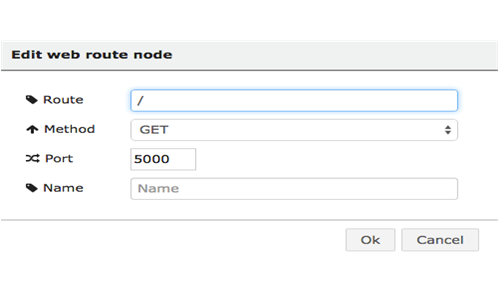
\includegraphics[width=0.4\textwidth]{figures/Web servers using Wyliodrin.png}
    \caption{Web servers using Wyliodrin}
\end{figure}

The payload goes either in the query string for the get method or in the upload data for post. The message is built on this payload, on two mandatory variables: res which stands for the response and req. which is the request. Without the last two, the server won't be able to provide a response.

\begin{figure}[ht]
    \centering
    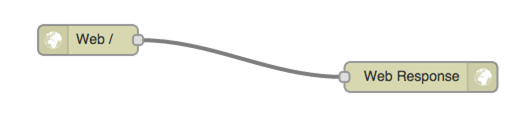
\includegraphics[width=0.4\textwidth]{figures/Webservers response.png}
    \caption{Webservers response diagram}
\end{figure}

The web response node: The message received by this node comes from one web node. For a web response the simple way is to make a redirection. Which means, in the redirect field, you can write the path to one of the static files and the browser will be sent to this page? On top of these, you will need the board's IP address which might not be public unless it is in the same network with the web server. 

\begin{figure}[ht]

\begin{subfigure}{0.5\textwidth}
    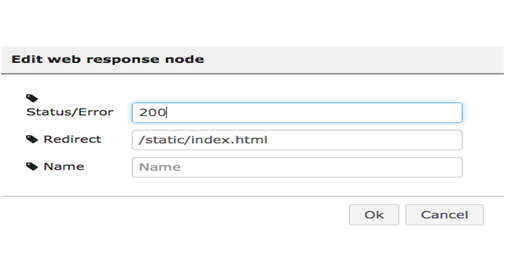
\includegraphics[width=0.9\linewidth, height=4cm]{figures/Webservers response using Wyliodrin.png}
    \caption{Webservers response using Wyliodrin}
\end{subfigure}
\begin{subfigure}{0.4\textwidth}
    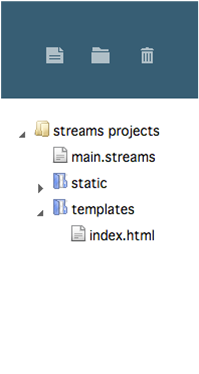
\includegraphics[width=0.9\linewidth, height=4cm]{figures/Webservers response files.png}
    \caption{Webservers response files}
\end{subfigure}

\caption{Webservers response}
\end{figure}

As a solution, IOT servers have a public address. The port for these servers can be either 80 for http or 443 for https. The user accesses the public page, through the IOT server which is connected to Wyliodrin as well as the board. Now the problem with the board and the web being in the same network is solved as both can communicate with Wyliodrin.  
Web templates: Just as for the static files, you will need a templates folder. This time, when you use the node, you don't need the whole path. You can only write the name of the file in the templates folder. What does the node do? It processes the response, meaning it loads the values plus the payload in it and sends it back to the browser. The values need to be in between two sets of curly brackets {{}}. Note that the values won't update unless the page is reloaded.  

\begin{figure}[ht]

\begin{subfigure}{0.5\textwidth}
    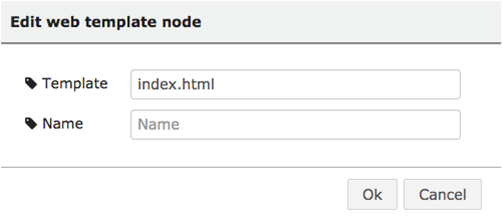
\includegraphics[width=0.9\linewidth, height=4cm]{figures/Edit Web Template Node.png}
    \caption{Edit Web Template Node}
\end{subfigure}
\begin{subfigure}{0.4\textwidth}
    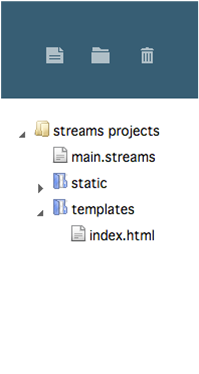
\includegraphics[width=0.9\linewidth, height=4cm]{figures/Edit Web Template Node Files.png}
    \caption{Web Template Node Files}
\end{subfigure}

\caption{Edit Web Template Node}
\end{figure}

\subsection{Web services}
A long time ago, the web services were more complicated. Now the application only requests the web server for the data, and it is the browser's job to rearrange it so that it is in the right format for the application.  
How to implement it into a Wyliodrin application? Using a simple web response and web server node, you send a static page to the user and each time you make a query, instead of a template, you use a web response node and send the payload to the browser, which can be a number, an object or anything else. 

\subsection{JQuery}
There is a library called JQuery, based on JavaScript, thus available in any browser, which can make function calls to the server.  
Case study: You have the following situation: you change the payload into a variable which stores values from a sensor. You want this variable to be shown in your web page. Practically, when an API gets called, what you will do, will be to make a get request to the server using the web address that you want with the URL /sensor. The web page will send values that you will store in a variable in your HTML file.  

\subsection{Web sockets}
A web socket is based on the http or https protocol. It builds a connection between the browser and the server, so that either one can send data. When the browser makes a request, the server recognizes the socket and doesn't close the connection. The two parties send the packages they need to send. If the server does not know how to work with sockets, the socket io will go back to querying.

\subsection{AngularJS}
AngularJS is a library through which you can build browser applications. In the next example, every web node will create a new socket and serve a static web page. If you include in the response a variable, and this variable changes, wyliodrin controller will be notified every time this kind of novelty appears and AngularJS will replace the old value of the variable with the new one, creating a dynamic web page.

\begin{figure}[ht]

\begin{subfigure}{0.5\textwidth}
    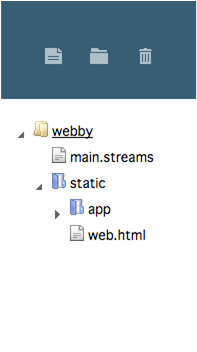
\includegraphics[width=0.9\linewidth, height=4cm]{figures/AngularJS files.png}
    \caption{AngularJS files}
\end{subfigure}
\begin{subfigure}{0.4\textwidth}
    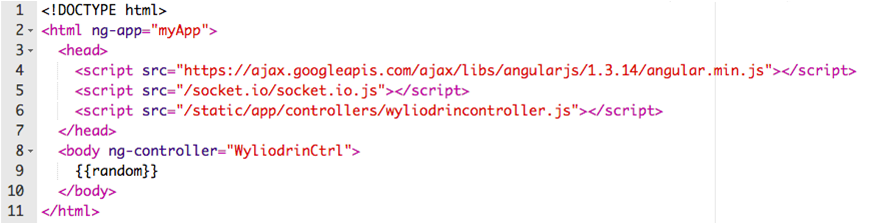
\includegraphics[width=0.9\linewidth, height=4cm]{figures/AngularJS in code.png}
    \caption{AngularJS in code}
\end{subfigure}

\caption{AngularJS files}
\end{figure}

\begin{figure}[ht]
    \centering
    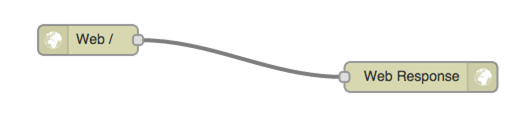
\includegraphics[width=0.4\textwidth]{figures/AngularJS files and web response.png}
    \caption{AngularJS files and web response}
\end{figure}


